\documentclass{report}
\usepackage{lipsum}
\usepackage{gensymb}
\usepackage{float}
\usepackage{graphicx} % Required for inserting images


\usepackage{cite}
\usepackage{caption}

\usepackage{graphicx}
\usepackage{svg}
\usepackage{xcolor}
\usepackage{tikz}
\usepackage{hyperref}
\usepackage{multirow}
\usepackage{enumerate}
\usepackage[shortlabels]{enumitem}
\usepackage{longtable}
\usepackage{array}
\usepackage{amsmath}
\usepackage{nomencl} % For nomenclature and acronyms
\makenomenclature % Activate nomenclature

\definecolor{lightblue}{HTML}{a0d8ef}

\title{Embedded System Security - Security Analysis of  Automotive In-Vehicle Networks Report} %title of the file

\begin{document}

%----------- Report information ---------

\logo{logos/ULB_round.png}
\uni{\textbf{Université Libre de Bruxelles}}
\ttitle{Security Analysis of  Automotive In-Vehicle Networks (CAN and Automotive Ethernet)} %title of the file
\subject{Embedded System Security} % Subject name
\topic{Project Report} % Topic name

\professor{Prof. \textsc{MÜHLBERG} Jan Tobias} % information related to the professor

\students{\textsc{Amanor} Deborah\\
          \textsc{Hassani} Mortaza} % information related to the students

%----------- Init -------------------

\buildmargins % display margins
\buildcover % create the front cover of the document
\toc % creates the table of contents

%------------ Report body ----------------
\section*{Contribution}
This project was a collaborative effort, with each team member contributing their expertise to ensure successful completion. In the initial phase, we jointly conducted a comprehensive literature review, analyzing several sources before shortlisting three key references that were most relevant to our research. Together, we formulated the research questions that guided the direction of the project. 

Deborah focused on researching Automotive IVN Security Issues, vulnerabilities and threat modelling, while Mortaza focused on Identifying use cases, existing security measures and emerging trends for securing CAN and Automotive Ethernet. Both team members worked collaboratively on drafting, refining, and finalizing the report to ensure the project's success.

\section*{Abstract}
\addcontentsline{toc}{section}{Abstract}
Automotive In-Vehicle Networks (IVNs) serve as the backbone for communication between various components and Electronic Control Units (ECUs) inside a vehicle's architecture. These enable seamless integration and/or operation of critical systems, such as powertrain, infotainment, advanced driver-assistance systems (ADAS) and safety mechanisms. However, the protocols used in IVNs, such as Controller Area Network (CAN) and Automotive Ethernet, at first place were designed with a focus on efficiency, reliability, and real-time communication rather than security. As a result, they lack robust mechanisms to protect against modern cyber threats. With the increasing connectivity of vehicles to external networks, such as the internet and mobile devices, the attack surface has expanded significantly, exposing vehicles to potential cyberattacks. This report provides a comprehensive analysis of the security challenges and vulnerabilities associated with CAN and Automotive Ethernet, studying some real-world attack scenarios, and proposes mitigation strategies to enhance the security of modern automotive systems.
\\
\\
\emph{\textbf{Keywords:} Automotive Ethernet, CAN, V2X, Security}

\section*{Introduction}
\addcontentsline{toc}{section}{Introduction}
With the shift towards software-defined vehicles, Autonomous vehicles and vehicle-to-everything (V2X) applications, there is an increasing demand for high bandwidth communication in the automotive domain. Over the years, automotive in-vehicle networks have comprised various protocols, ranging from high bandwidth, fault-tolerant ones supporting safety-critical applications such as Powetrain and braking system,  to low bandwidth protocols supporting secondary applications like HVAC and body control module (BCM).

The Controller Area Network (CAN)  has been the backbone of IVNs, providing reliable and deterministic communication for critical functions like engine control and braking systems. However, as vehicles become increasingly connected, CAN's limitations in terms of bandwidth and lack of built-in security pose significant challenges.

Automotive Ethernet has emerged as a promising alternative, offering higher bandwidth to support advanced applications like infotainment, telematics, and ADAS.  Despite its lower bandwidth, CAN remains a vital component of IVNs, due to its deterministic and reliable timing properties.

Both protocols, however, face unique security challenges. CAN, as a legacy protocol, was not designed with modern security threats in mind, while Automotive Ethernet inherits vulnerabilities from traditional IT Ethernet, exposing vehicles to a broader attack surface. This research focuses on analyzing the security issues in these two critical in-vehicle network protocols.

\section{Problem Statement}
In-Vehicle Networks (IVNs) are critical for communication between Electronic Control Units (ECUs) and other components within the vehicle's Electrical/Electronic (EE) architecture. They support both onboard communication and external connectivity with offboard services. However, existing protocols, particularly CAN and Automotive Ethernet (AE), exhibit significant security vulnerabilities.
Modern intelligent vehicles face increasing threats as adversaries exploit these vulnerabilities to compromise vehicle safety. Emerging technologies such as Vehicle-to-Everything (V2X) communication and over-the-air (OTA) updates further expand the attack surface, introducing new challenges in ensuring the security and privacy of vehicle data. Given the safety-critical nature of the automotive domain, addressing these vulnerabilities is an urgent priority, hence the goal of our research.

% \begin{figure}[h]
%     \centering
%     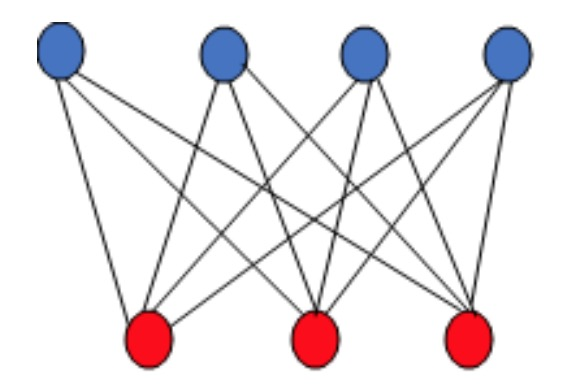
\includegraphics[width=0.25\textwidth]{figures/1.jpg}
%     \caption{biclique with m=4 and n=3}
%     \label{fig:biclique with m=4 and n=3}
% \end{figure}
% \nomenclature{ABC}{Abbreviation Example}

\subsection{Research Goal}
\begin{enumerate}
    \item Analyze the vehicle EE architecture trend:
    \begin{itemize}
        \item Explore how future EE systems integrate CAN and AE to meet safety-critical and bandwidth-intensive needs.
    \end{itemize}
    \item Assess vulnerabilities in CAN and Automotive Ethernet and the several ways they could be exploited including potential use cases.
    \item Propose Security Measures
    \begin{itemize}
        \item Explore how security zoning and defense-in-depth can mitigate these threats.
        \item Discuss Intrusion Detection Systems (IDS) for anomaly detection and their limitations.
    \end{itemize}
    \item Investigate emerging trends, such as the use of blockchain for IVN security.
\end{enumerate}


\subsection{Scope of Study}
The automotive IVN, is made up of several networking protocols, CAN, CAN-FD, Automotive Ethernet, Flexray, LIN and MOST. However, for the scope of this project we wiil focus on CAN and Automotive Ethernet. This decision is based on the following considerations:

\begin{enumerate}
    \item \textbf{Flexray:} Although it offers higher bandwidth and fault tolerance compared to CAN, its high implementation cost has limited its adoption. Additionally, the growing adoption of Automotive Ethernet is gradually phasing out FlexRay as the preferred high-bandwidth solution.
    \item \textbf{LIN:} LIN is designed for low-bandwidth, cost-effective applications and is not used for safety-critical systems, making it less relevant to the scope of this project.
    \item \textbf{MOST:} MOST is primarily used for multimedia and infotainment systems, which do not form part of the project's focus on safety-critical and core operational networks.
\end{enumerate}

\section{Methodology}
To achieve the goal of this research, we adopted a structured and systematic approach to gain a thorough understanding of the domain (vehicle EE architecture and IVN protocols), and the associated security challenges. By conducting a comprehensive literature study and evaluating vulnerabilities,  our research aims to address the critical security gaps in modern IVNs and evaluate the solutions being implemented to mitigate them.

Our methodology consists of four key steps:

\begin{enumerate}
    \item \textbf{Literature Review:} We conduct a thorough review of existing literature to establish a deep understanding of the current vehicle EE architecture, IVN protocols, and associated security challenges.
    \item \textbf{Vulnerability Assessment:} We identify specific weaknesses in CAN and AE protocols that adversaries could exploit, using both theoretical and practical perspectives.
    \item \textbf{Analysis of Real-World Attacks:} We connect theoretical vulnerabilities to practical attack scenarios, providing a clear understanding of their implications on real-world systems.
    \item \textbf{Mitigation Strategies:} We evaluate and propose mitigation solutions based on identified vulnerabilities and attack surface.
\end{enumerate}

\subsection{Limitations of Methodology}
Given more time, we would have addressed other IVN protocols, such as FlexRay and LIN, to provide a more holistic view of Automotive IVN security. Additionally, we would have delved deeper into the security challenges posed by vehicular external networks, such as cellular and Wi-Fi, to address software-defined vehicle challenges comprehensively. Furthermore, a more detailed threat modeling of the attack landscape would have been developed.


\subsection{Literature Study}
The study focused on reviewing the following key papers:

\begin{enumerate}
    \item \textbf{Security Issues with In-Vehicle Networks, and Enhanced Countermeasures Based on Blockchain} by Narayan Khatri et al.
    \begin{itemize}
        \item Compares the security vulnerabilities of the various IVNs and proposes how blockchain can be applied for secure communication.
    \end{itemize}
    \item \textbf{In-Vehicle Communication Cyber Security: Challenges and Solutions} by Rajkumar Singh Rathore et al
    \begin{itemize}
        \item Identifies key challenges in CAN and AE, and proposes security solutions such as IDS.
    \end{itemize}
    \item \textbf{Security Analysis of Ethernet in Cars} by Ammar Talic KTH, Sweden.
    \begin{itemize}
        \item Focuses on vulnerabilities in Automotive Ethernet.
    \end{itemize}
\end{enumerate}

\subsection{Research Questions}
To guide the literature review, the following research questions were posed:

\begin{itemize}
    \item \textbf{RQ1:} What is the current vehicle EE architecture and what is the future trend?
    \item \textbf{RQ2:} How are these IVNs (CAN and AE) enablers for the Vehicle EE architecture?
    \item \textbf{RQ3:} What are the key attack surfaces and vulnerabilities of CAN and AE?
    \item \textbf{RQ4:} What trade-offs are associated with implementing security measures?
    \item \textbf{RQ5:} How does fuzzing reveal vulnerabilities in CAN and AE?
    \item \textbf{RQ6:} What security measures are currently in use for CAN and AE?
\end{itemize}

\subsection{Structure of the Report}
The report is organized into the following sections

\begin{description}[leftmargin=!,labelwidth=\widthof{\bfseries Section 8:}]
    \item[Section 3:] Provides the background of the various vehicle EE architectures and their evolution to date, along with a brief description of the IVN protocols used within the vehicle EE architecture.
    \item[Section 4:] Details the security issues and vulnerabilities found in CAN and AE.
    \item[Section 5:] Analyzes three use cases of real-world attacks carried out on automotive vehicles and includes threat modeling for all.
    \item[Section 6:] Discusses security mitigations based on our proposals and recommendations from other researchers.
    \item[Section 7:] Addresses and answers the research questions posed for the study.
    \item[Section 8:] Concludes the study with final thoughts and recommendations.
\end{description}

\section{Background}
This section presents study of available technologies used in vehicle communication.\cite{kaiwartya2016internet}

\subsection{The Vehicle E/E architecture}
The E/E system architecture of automotive vehicles has evolved over the years from a flat backbone architecture where the backbone networking technology was CAN-based. As the number of ECUs connected to the backbone expanded and additional subnets and sub systems were introduced, data transport on the backbone became a bottleneck and as such the flat backbone architecture evolved to domain distributed and domain centralized architectures and now the future is zonal architecture.\cite{zerfowski2019functional}

\subsubsection{Domain Distributed E/E Architecture}
In this architecture, Electronic Control Units (ECUs) with similar functionalities are grouped into functional domains such as Telematics, Powertrain, Body, and Chassis. ECUs in different domains communicate with each other via a central gateway.

\subsubsection{Domain Centralized E/E Architecture}
Similar to the domain distributed architecture, ECUs are grouped into functional domains. However, in this setup, each domain has a Domain Control Unit (DCU) which manages and coordinates the operations within the domain. For inter-domain communication, Automotive Ethernet or CAN is used as the backbone. Intra-domain communication can occur via different networks, helping to segment and enhance security within the vehicle.

\subsubsection{Zonal Architecture}
The zonal architecture represents the future of vehicle E/E architecture, introducing high-performance compute nodes. This architecture supports the concept of the software-defined vehicle, where new functionalities are added through over-the-air updates rather than by replacing or adding ECUs. Key components include vehicle servers and zonal gateways, which facilitate efficient and flexible communication across the vehicle.

\subsection{In-Vehicle Networking Technologies}
The in-vehicle network is an enabler for the vehicle E/E architecture. It facilitates the transport of data among several ECUs within the same domain as well as between different domains. In-vehicle communication protocols in the E/E system are heterogeneous, consisting of CAN, Automotive Ethernet, LIN, Flexray and MOST protocols. 

For communication between onboard and offboard services, a combination of both wireless and wired networking technologies is used. Wireless technologies such as Wi-fi, cellular networks and Bluetooth enable connectivity to cloud services  this is usually housed in the telematics domain. Whereas classical Ethernet, 100 Base-TX or CAN is used for On-Board Diagnostics (OBD).

\subsubsection{CAN}
CAN is the most widely used in-vehicle networking protocol. It is a bus-based technology where all ECUs are attached and share the same wiring. CAN is a broadcast technology where every node can transmit and receive frames over the medium. To prevent collisions, the arbitration method is used where the node with the highest priority is allowed to communicate on the bus. The CAN bus consists of two twisted pair wires known as the \emph{CANH}(CAN High) and \emph{CANL}(CAN Low)  which enhances immunity to EMI. Classical CAN supports data rates up to 1 Mbps and a payload of 8 bytes. However, a better version of CAN exists with improved data rates of 8 Mbps and an extended payload of 64 bytes.

\subsubsection{Automotive Ethernet}
Automotive Ethernet is a special type of Ethernet that fulfils the stringent requirements of EMC in the automotive environment [3]. It is also designed to ensure reliable and deterministic communication, which is crucial for safety-critical applications and real-time communication through the use of the protocols, AVB and TSN.

Automotive Ethernet can currently support data rates of up to 10 Gbps[3], a significant improvement compared to the traditional in-vehicle networking protocols. This high data rate capability coupled with traffic prioritization and shaping (QoS)enables the support of advanced automotive applications such as autonomous driving and V2X . The AE technology is based on switches which allows efficient data routing and minimizes latency making it suitable for the modern vehicle.

\subsubsection{LIN}
LIN is a low-cost serial communication protocol. Unlike CAN being a multi master communication protocol, LIN is a single master networking protocol. The data rate is up to 20 kbps making it a useful technology for low-speed, non-safety critical tasks such as comfort clusters, doors and seat

\subsubsection{FlexRay}
FlexRay evolved as an alternative for more demanding tasks which needed better performance than CAN could provide. It operates at a higher data rate of 10 Mbit/s and is used for applications such as Drive-by-wire, active suspension, and adaptive cruise control. FlexRay is an innovative communication protocol which combines event-driven and deterministic communication with static and dynamic segments. A static segment is reserved for deterministic data, while a dynamic segment is used for priority based event-driven communication
\subsubsection{MOST}
MOST is a high-speed protocol developed for infotainment and media oriented communication. Its maximum data rate is 24.8 Mbit/s and it can support up to 64 nodes. However because of the adoption of Automotive Ethernet, the use of most is decreasing.

Below is a table showing the various protocols and their bandwidth;

\begin{table}[H]
    \centering
    \begin{tabular}{|>{\raggedright\arraybackslash}p{3cm}|>{\raggedright\arraybackslash}p{4cm}|}
    \hline
    \textbf{Protocol} & \textbf{Bandwidth} \\
    \hline
    CAN & 125 Kbps - 1 Mbps \\
    \hline
    LIN & 1 Kbps - 20 Kbps \\
    \hline
    Flexray & 10 Mbps \\
    \hline
    MOST & 24 Mbps \\
    \hline
    Automotive Ethernet & 100 Mbps - 10 Gbps \\
    \hline
    \end{tabular}
    \caption{Table showing In-vehicle networking protocols and their bandwidths}
    \label{tab:protocols}
    \end{table}
\section{Security Issues and Vulnerabilities }
Vehicles have relatively long life cycles, during which attack patterns and vulnerabilities evolve, exposing them to new and emerging threats.\cite{talic_security} This section outlines the major attack surfaces and vulnerabilities associated with the CAN and Automotive Ethernet AE networks

\subsection{Attack Surface of CAN and AE}
Adversaries target specific entry points to exploit vulnerabilities in CAN and Automotive Ethernet networks. These attack surfaces can be categorized as follows;
\subsubsection{Remote/offboard attack}
These attacks target external communication interfaces and systems, primarily through the telematics unit. The telematics unit is the domain in the vehicle that consists of wireless communication interfaces such as:

\begin{enumerate}
    \item \textbf{Wi-Fi:} Attackers can exploit unsecured or poorly configured vehicle Wi-Fi networks to gain unauthorized access to in-vehicle systems.
    \item \textbf{Bluetooth:} Vulnerable to pairing exploits or unauthorized connections, allowing attackers to manipulate connected systems.
    % \item \textbf{Wireless Key Fobs:} Replay or spoofing attacks, such as the TeslaX attack, can enable unauthorized access or control of the vehicle. Additionally, the constant power-on state of certain ECUs, like those in keyless comfort entry systems, can be used as an attack vector, even when the vehicle is parked and locked.
    \item \textbf{Cellular Networks:} Used for vehicle connectivity and over-the-air updates, these networks can be targeted to infiltrate telematics systems.
\end{enumerate}

\subsubsection{Physical/Onboard attacks}
These require physical access to the vehicle through the following interfaces:

\begin{enumerate}
    \item \textbf{OBD-II Port:} Used for diagnostics, this port can be exploited to inject malicious CAN messages.\cite{klinedinst2016onboard}
    \item \textbf{USB Ports:} Unsecured USB interfaces can be used to upload malware.
    \item \textbf{Electric Vehicle (EV) Charging Ports}
    \item \textbf{Ethernet Switches:} Attackers can target AE switches to intercept, reroute, or block critical data flows within the network.
\end{enumerate}

\subsubsection{Hybrid Attacks}
Adversaries often combine remote and physical attack vectors.  An attacker might exploit a vulnerability in the telematics unit remotely and then gain deeper access during physical interaction with the vehicle for further post exploitation.
Figure~\ref{fig:Hybrid Attacks}  illustrates a hybrid attack scenario where adversaries combine remote and physical attack vectors to exploit vulnerabilities in a vehicle's telematics unit. Initially, the attacker gains remote access, then physically interacts with the vehicle to deepen their exploitation and compromise critical systems.
\begin{figure}[h]
    \centering
    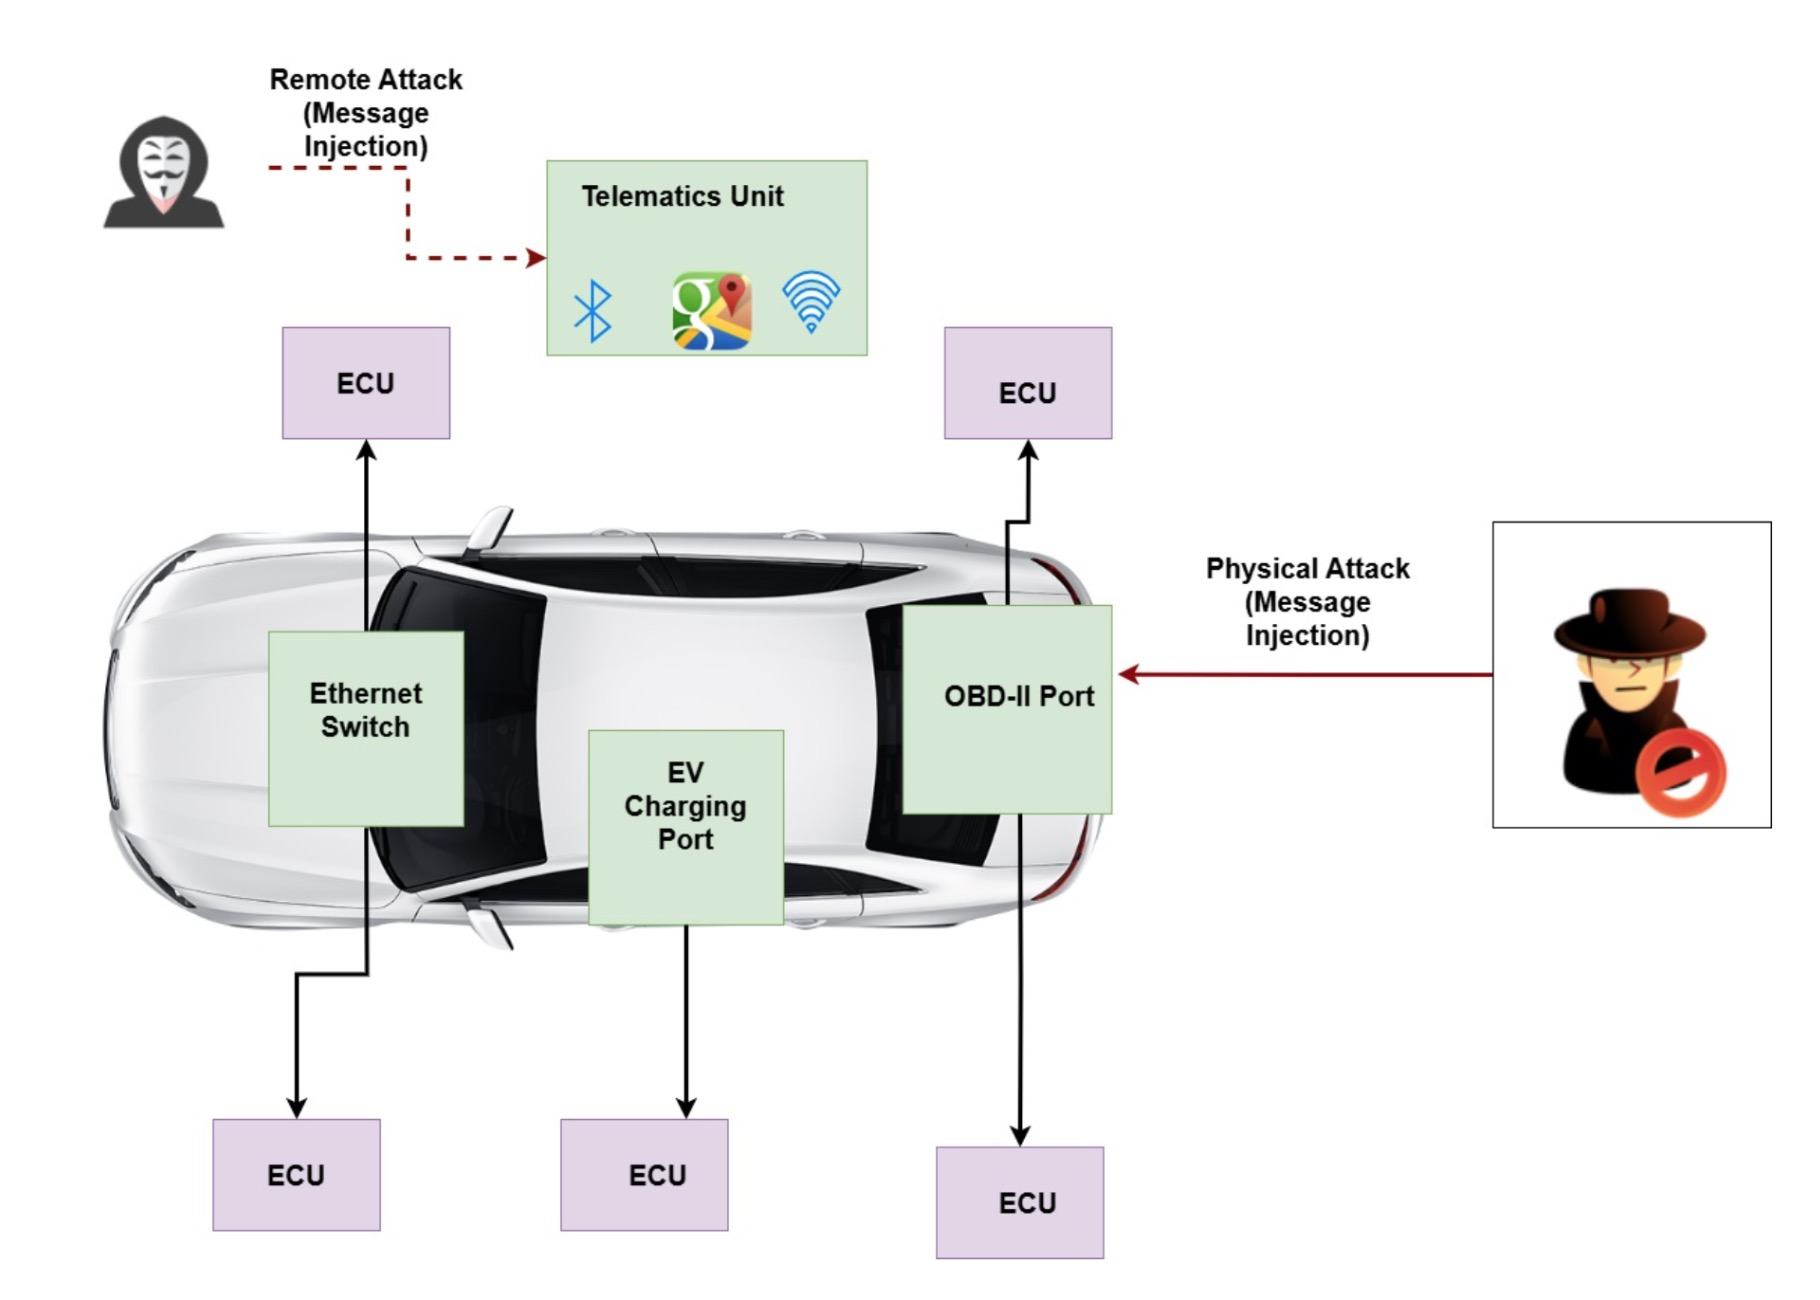
\includegraphics[width=0.8\textwidth]{figures/hybrid.jpg}
    \caption{Hybrid Attacks}
    \label{fig:Hybrid Attacks}
\end{figure}

\subsection{Vulnerabilities in CAN}
CAN a legacy protocol, was developed without considering modern security threats, making it inherently vulnerable to various attacks. Below are the major vulnerabilities identified in the CAN network:

\subsubsection{ID-Based Arbitration}
CAN uses Carrier Sense Multiple Access with Collision Detection (CSMA/CD) to manage message collisions. Arbitration is based on message IDs where ECUs with lower message ID have higher priority and are allowed to transmit first. Attackers can exploit this mechanism to execute a Denial-of-Service (DoS) attack by injecting high-priority messages that dominate the bus blocking legitimate ECUs to transmit.

\subsubsection{Lack of Authenticated Messages}
The CAN frame has no field for sender or receiver information to determine a legitimate communicating device. Thus, the authenticity of the message cannot be guaranteed in CAN networks, allowing attackers to inject malicious messages into the network.

\subsubsection{Lack of Confidentiality}
Since CAN is a broadcast Network, all nodes receive data that is transmitted hence, a malicious ECU has the tendency to eavesdrop and intercept data transmitted on the bus. This is because messages are not encrypted in CAN leading to a lack of confidentiality.

\subsection{Common CAN Bus Attacks}
Exploiting these vulnerabilities can lead to the execution of the following attacks on the CAN bus:

\begin{enumerate}
    \item \textbf{Denial-of-Service (DoS) attacks:} By exploiting the arbitration mechanism, attackers inject high-priority messages to dominate the bus, preventing legitimate ECUs from communicating. Critical vehicle systems are disrupted, potentially compromising safety.
    \item \textbf{Fuzzing Attacks:} Attackers send random or malformed CAN messages to test how ECUs respond to unexpected inputs. This can reveal weaknesses in ECU software and hardware, causing crashes or unexpected behavior.
    \item \textbf{Replay Attacks:} Replay attacks occur when an attacker intercepts legitimate CAN messages and retransmits them at a later time, potentially causing unauthorized actions or disruptions. Since CAN cannot differentiate between original and replayed messages, this can lead to unintended consequences, such as unlocking doors. The wireless key fob functionality is particularly vulnerable to this type of attack, making it a common target for exploitation.
    \item \textbf{Impersonation or Spoofing attacks:} By pretending to be a legitimate ECU, attackers inject malicious frames into the network. This can manipulate the vehicle system, such as deploying airbags or tampering with engine performance.
\end{enumerate}

\subsection{Vulnerabilities in Automotive Ethernet}
Automotive ethernet inherits vulnerabilities from traditional IT ethernet. The vulnerabilities are non-exhaustive and only a few are captured in this study. Some of the attack patterns in AE have similar characteristics to the ones in CAN networks, e.g., replay attacks and spoofing, DoS
The primary categories of vulnerabilities in Automotive Ethernet Networks include:
\subsubsection{Unauthorized Joins}
Any device can connect to an unconnected port on the switch. This means that anyone with physical access to the switch can eventually have access to the network and can communicate in several ways such as VLAN hopping where a user may create frames to bypass VLAN segmentation.

\subsubsection{Spoofing attacks}
\begin{itemize}
    \item \textbf{MAC Spoofing:} Attackers can change their device’s MAC address to mimic another device on the network, gaining unauthorized access and potentially disrupting network services.
    \item \textbf{DHCP Spoofing:} Attackers can set up a rogue DHCP server to provide incorrect IP addresses to devices, redirecting traffic to malicious nodes.
    \item \textbf{IP Spoofing:} Attackers can send IP packets from a false (or spoofed) source address, making it appear as though the packets are coming from a trusted source.
\end{itemize}

\subsubsection{Man-in-the-middle attacks}
In the Man-in-the-Middle (MitM) attack, the attacker intercepts communication between two ECUs or nodes, eavesdropping or altering the transmitted data without their knowledge. This can lead to the exposure of sensitive information or the injection of malicious data into the communication stream.

\subsubsection{MAC Table flooding}
Switches maintain a MAC table to map MAC addresses to switch ports. In a MAC table flooding attack, an attacker floods the switch with a large number of frames, each with a different source MAC address. This can overflow the MAC table, causing the switch to broadcast all frames to all ports, effectively turning the switch into a hub and allowing the attacker to sniff all network traffic.

\subsubsection{ARP table poisoning}
Attackers send fake ARP messages to associate their MAC address with the IP address of a legitimate device. This allows them to intercept, modify, or stop data intended for that device.

\subsection{Threat Modeling Using STRIDE}
The STRIDE framework using the Microsoft Threat Modelling Tool was used for the threat modeling of CAN and Automotive ethernet. This approach allowed us to identify potential threats and assess their impact and exploitation methods. 

\subsubsection{Assumptions}
In our threat model, we made the following assumptions:
\begin{itemize}
    \item Vehicles using only CAN
    \item Vehicles using only Automotive Ethernet
    \item Vehicles using a combination of both
    
\end{itemize}

\subsubsection{Domain Segmentation}
For the purposes of this threat model, the analysis focused on five key domains within the vehicle system:
\begin{enumerate}
    \item ADAS (Advanced Driver Assistance Systems)
    \item Powertrain
    \item EV-ECU (Electric Vehicle - Electronic Control Unit)
    \item Telematics
    \item Infotainment
\end{enumerate}

\subsubsection{Trust Zones}
The system was segmented into three trust zones:
\begin{enumerate}
    \item \textbf{Untrusted Zone:} Includes external elements such as user phones and cloud services that access vehicle services like OTA (Over-The-Air) updates. These elements are considered high-risk.
    \item \textbf{Exposed Zone:} Hosts components that connect directly with elements in the untrusted zone. This zone serves as the intermediary layer, bridging external networks with the vehicle's internal systems.
    \item \textbf{Critical Zone:} Contains components responsible for safety-critical functions within the vehicle.
\end{enumerate}
\begin{figure}[H]
    \centering
    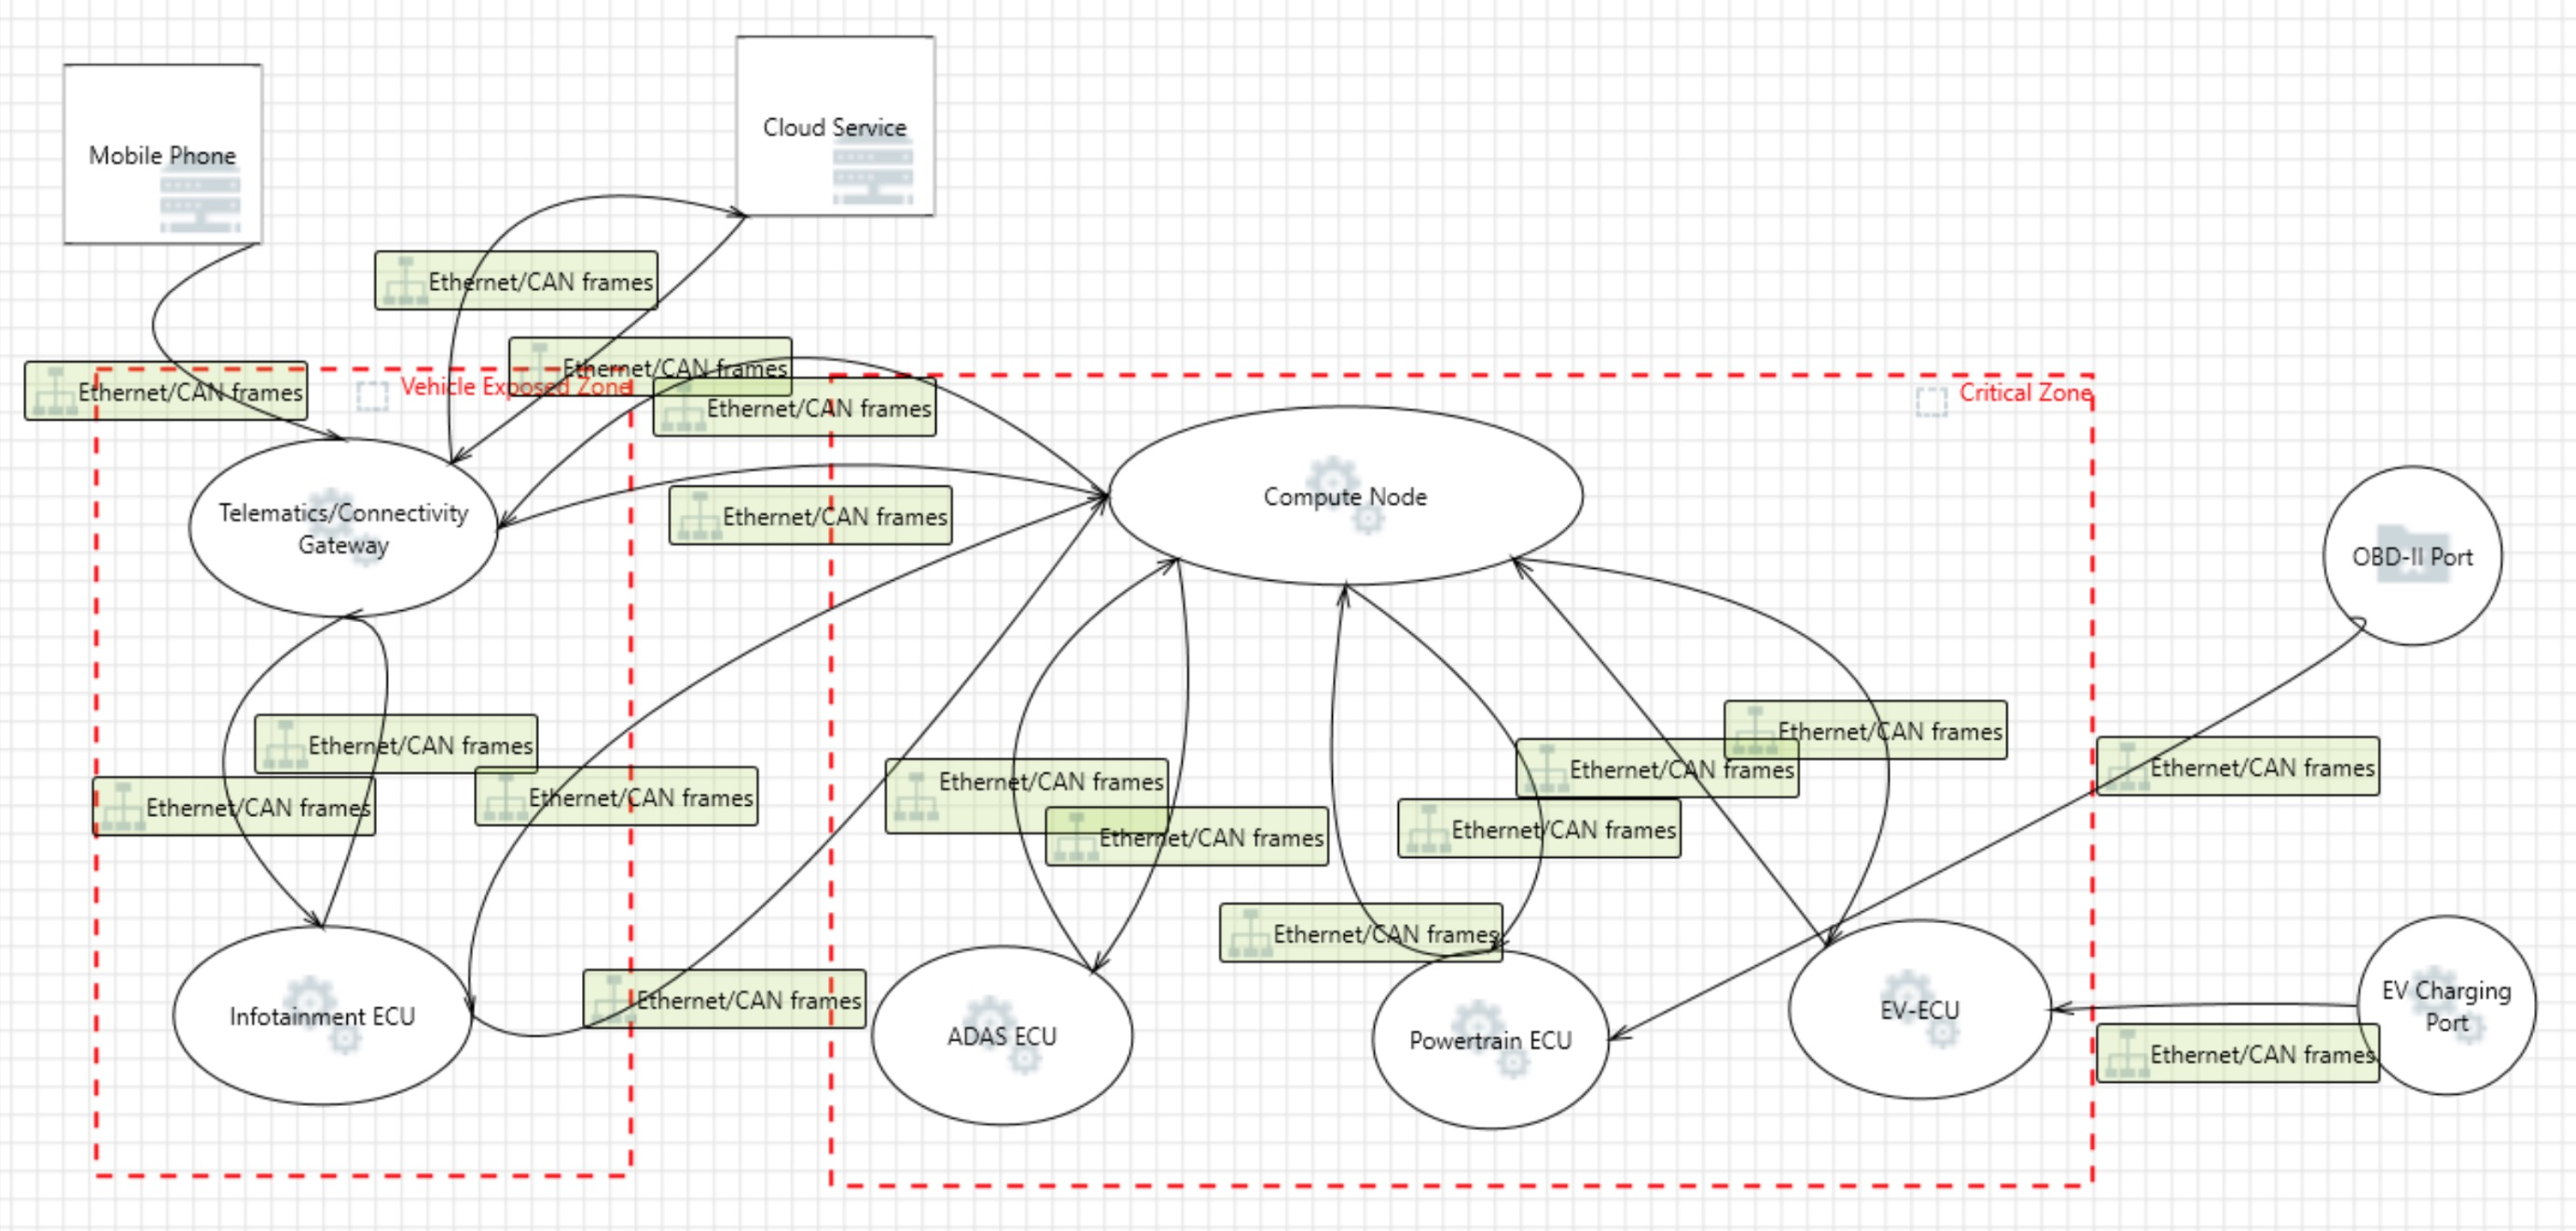
\includegraphics[width=0.8\textwidth]{figures/zone.jpg}
    \caption{Stride Threat Model of CAN and Automotive Ethernet in Vehicle system}
    \label{fig:Stride}
\end{figure}

Below is the STRIDE table These threats represent common yet critical vulnerabilities in both Automotive Ethernet and CAN. Each threat aligns with STRIDE categories and highlights realistic attack vectors that could compromise IVN security;
\begin{longtable}{|>{\raggedright\arraybackslash}p{2cm}|>{\raggedright\arraybackslash}p{4cm}|>{\raggedright\arraybackslash}p{3cm}|>{\raggedright\arraybackslash}p{3cm}|>{\raggedright\arraybackslash}p{3cm}|}
    \hline
    \textbf{Threat Type} & \textbf{Description} & \textbf{Assets Affected} & \textbf{Exploitation Method} & \textbf{Example Scenario} \\
    \hline
    \endfirsthead
    \hline
    \textbf{Threat Type} & \textbf{Description} & \textbf{Assets Affected} & \textbf{Exploitation Method} & \textbf{Example Scenario} \\
    \hline
    \endhead
    \hline
    \endfoot
    \hline
    \endlastfoot
    Spoofing & An adversary may gain unauthorized access to resources by impersonating a legitimate ECU or gateway. & ECUs, Gateways & Sending falsified CAN/Ethernet packets mimicking legitimate nodes. & An attacker spoofs an ECU to disrupt powertrain functionality. \\
    \hline
    Spoofing & An adversary can exploit the gateway to mimic external entities like mobile devices. & Gateways, Mobile Devices & Using a rogue mobile app to spoof a legitimate device communicating via V2X. & A malicious app sends fake location data to manipulate navigation. \\
    \hline
    Tampering & An adversary may alter Ethernet frames or CAN messages in transit. & CAN Bus, Ethernet Frames & Man-in-the-middle attack modifies critical commands or sensor data. & Modifying braking system commands in CAN messages. \\
    \hline
    Tampering & An adversary may inject false diagnostic messages via the OBD-II port. & CAN Bus, Diagnostic Tools & Exploiting physical access to the OBD-II port to inject tampered commands. & Overwriting firmware using false diagnostic instructions. \\
    \hline
    Information Disclosure & An adversary can gain access to sensitive unencrypted data flowing between nodes. & Ethernet Frames, CAN Bus & Using sniffing tools to intercept network traffic. & Capturing unencrypted CAN messages to reverse-engineer ECU commands. \\
    \hline
    Information Disclosure & An adversary may intercept OTA update data during transmission to the vehicle. & Cloud Services, Gateways & Exploiting lack of encryption in OTA updates to obtain sensitive data. & An attacker captures vehicle firmware updates from the cloud. \\
    \hline
    Denial of Service (DoS) & Flooding the CAN Bus or Ethernet network with high-priority messages, disrupting legitimate communication. & CAN Bus, Ethernet Switch & Overloading the network to prevent normal operation of ECUs. & A malicious device floods the CAN Bus, disabling ADAS functionality. \\
    \hline
    Denial of Service (DoS) & Exploiting vulnerabilities in the telematics gateway to disrupt communication between cloud and vehicle systems. & Telematics Gateway, Cloud Services & Sending malformed packets to crash the gateway or block data flow. & An attacker crashes the telematics gateway, disabling V2X communication. \\
    \hline
    Elevation of Privilege & An adversary may gain access to higher-privileged functions by exploiting gateway or ECU vulnerabilities. & Gateways, ECUs & Exploiting unpatched vulnerabilities or weak access control mechanisms. & Gaining control over the ADAS system by exploiting a gateway flaw. \\
    \hline
    Elevation of Privilege & An attacker may use unprotected diagnostic interfaces to gain access to critical vehicle systems. & OBD-II Port, ECUs & Exploiting the lack of authentication on the OBD-II interface. & Using the OBD-II port to disable vehicle security features like alarms. \\
    \hline
    \caption{Summary of Threats Identified in CAN and Automotive Ethernet Using STRIDE}
    \label{tab:threat_analysis}
\end{longtable}

\section{Use Case Scenarios}

In this section, we outline a use case relevant to our study.

% \subsection{Tesla X Wireless key fob  attack}
% \textbf{Brief Description}\\
% Researchers in KU leuven previously hacked the keyless entry of the me tesla model s. Although tesla improved the security in the new model, They found additional ways to bypass the tesla model . The same researchers hacked the Tesla Model S keyless entry system and now detail how the security measures implemented in the more recent Tesla Model X can be bypassed. They demonstrate how the battery powered Tesla Model X priced at over \$100.000 US can be stolen in a few minutes. The  Attack flow is shown below:
% \begin{figure}[H]
%     \centering
%     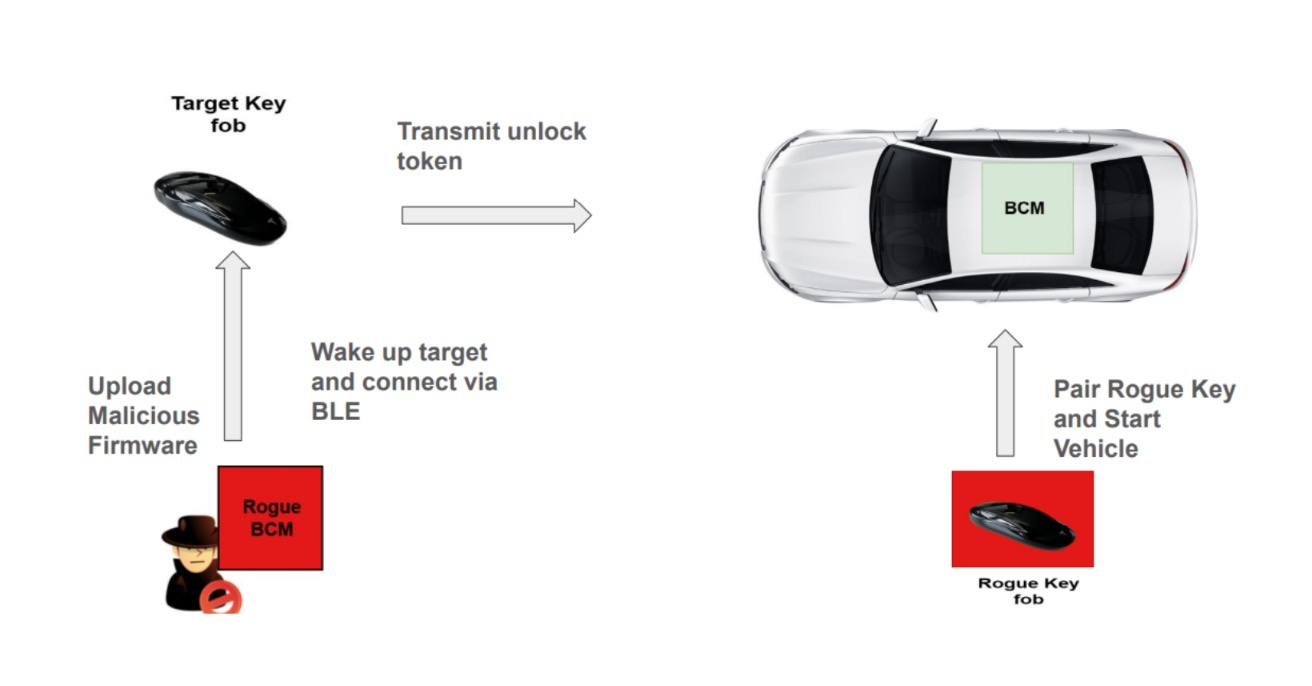
\includegraphics[width=0.8\textwidth]{figures/tesla.jpg}
%     \caption{Tesla X Wireless key fob  attack}
%     \label{fig:Tesla X Wireless key fob  attack}
% \end{figure}
% \textbf{Identified issues}\\
% First, the Model X key fobs lack what's known as "code signing" for their firmware updates. Tesla designed its Model X key fobs to receive over-the-air firmware updates via Bluetooth by wirelessly connecting to the computer inside a Model X.

\subsection{2014 Jeep Cherokee Attack}
The 2014 Jeep Cherokee attack by researchers Charlie Miller and Chris Valasek highlighted critical vulnerabilities in modern automotive in-vehicle networks (IVNs).\cite{valasek2014survey} This research demonstrated how adversaries could exploit weaknesses in both the CAN bus system and the connected Uconnect infotainment system, to compromise vehicle safety and functionality exploitation.
\subsubsection{overview of The Attack}
The researchers remotely accessed the Jeep Cherokee through its Uconnect infotainment system,  via cellular network exploiting its lack of secure communication protocols. This entry point allowed them to bridge the gap between the vehicle's external connectivity and its internal CAN bus, enabling them to inject malicious commands and manipulate various vehicle systems. The attack highlighted the growing attack surface being a major threat to the  in-vehicle network.

\subsubsection{Threat Analysis}
\begin{itemize}
    \item \textbf{ID-Based Arbitration Exploitation:} Attackers injected high-priority malicious messages, leading to Denial of Service (DoS) and blocking legitimate ECUs from communication.
    \item \textbf{Lack of Authentication:} Allowed unauthorized access to send commands to the CAN bus, leading to unsafe vehicle control (e.g., disabling brakes, manipulating acceleration).
    \item \textbf{Lack of Confidentiality:} Broadcast nature of the CAN bus enabled interception and injection of malicious messages.
    \item \textbf{Remote Entry via Uconnect:} Exploited vulnerabilities in AE to gain access to the CAN network, showcasing a hybrid attack scenario.
\end{itemize}
This attack demonstrated how interconnected vehicle systems can be exploited to gain deeper access, emphasizing the need for stringent security measures in in-vehicle networks.

\section{Security Mitigations and Recommendations}
\begin{enumerate}
    \item \textbf{Intrusion Detection Systems (IDS):}
    IDS play a critical role in monitoring network traffic for abnormal patterns or unauthorized activities.\cite{rathore2022invehicle} For CAN networks, anomaly-based IDS detect deviations from typical message patterns, such as sudden high-priority messages indicative of Denial-of-Service (DoS) attacks. In AE, signature-based IDS can identify known vulnerabilities, such as MAC spoofing or Man-in-the-Middle (MitM) attacks, ensuring timely detection and response. \cite{Evaluationframe}

    \item \textbf{Firewalls:}
    Firewalls act as a barrier between critical in-vehicle networks and external interfaces. For AE, firewalls are deployed at gateways to filter malicious traffic and enforce rules that limit communication to authorized systems. This segmentation reduces the risk of remote exploits spreading across network domains.

    \item \textbf{Deep Packet Inspection (DPI):}
    DPI enhances network security by inspecting the content of data packets beyond basic header information. For AE, DPI helps detect malicious payloads, unauthorized data, or malformed packets that could compromise ECUs or vehicle functionality.

    \item \textbf{MACsec:}
    Media Access Control Security (MACsec) is an IEEE 802.1AE standard that provides data integrity and encryption for Ethernet networks. In AE, MACsec ensures that communication between switches and devices is both confidential and tamper-proof, protecting against spoofing and MitM attacks.

    \item \textbf{Security Zones:}
    Security zoning involves segmenting networks into isolated domains based on their functionality and criticality. For instance, CAN-based safety-critical systems (e.g., braking) can be separated from AE-based infotainment or telematics domains. This minimizes the impact of an attack on one domain from affecting others.

    \item \textbf{Secure Boot:}
    Secure Boot ensures that only authorized and verified software can run on vehicle ECUs. By validating digital signatures during the startup process, Secure Boot prevents attackers from deploying malicious firmware, safeguarding both CAN and AE environments.

    \item \textbf{Port Security:}
    Port security restricts access to Ethernet switches by allowing only authorized devices to connect. In AE networks, port security can mitigate unauthorized joins or MAC address spoofing, enhancing control over physical access points.

\end{enumerate}

\subsection{Emerging Future Trends For Securing IVNs}

\subsubsection{Blockchain Technology}
Blockchain offers a decentralized and tamper-proof mechanism for securing in-vehicle communications and data exchanges.\cite{khatri2021security} By creating immutable logs of network activity, blockchain can help:
\begin{itemize}
    \item Ensure message integrity by validating data exchanged between ECUs.
    \item Detect unauthorized changes by maintaining a transparent history of events.
    \item Facilitate secure over-the-air (OTA) updates through trusted distributed networks. Blockchain's inherent resilience to single points of failure makes it a promising solution for safeguarding critical IVN components like CAN and AE against spoofing, replay, and tampering attacks.

\end{itemize}

\subsubsection{Zero Trust Architecture (ZTA)}
ZTA shifts the security paradigm by assuming that no device or user within a network is inherently trustworthy. In the context of automotive IVNs, ZTA principles can be applied to:
\begin{itemize}
    \item Authenticate and authorize every interaction within the network, regardless of its origin.
    \item Limit access to critical systems through micro-segmentation and strict access controls.
    \item Continuously monitor and assess devices for anomalies, ensuring real-time threat detection. By adopting ZTA, automakers can reduce the risk of lateral movement in attacks and enhance the overall security of both legacy (CAN) and modern (AE) networks.

\end{itemize}

These  technologies hold significant potential to transform the security landscape of in-vehicle networks, addressing evolving threats and ensuring robust protection for next-generation vehicles.

\section{Discussion and Analysis}

\subsection{Research Questions Answers}
\begin{itemize}
    \item \textbf{RQ1: What is the current vehicle EE architecture and what is the future trend?}
        \begin{itemize}
            \item Currently, most automotive OEMs use a domain-based architecture where Electronic Control Units (ECUs) with similar functionalities are grouped into functional domains. Each domain has a domain control unit that acts as a gateway for communication between different domains. This interdomain communication happens through the gateway.

            \item With the shift towards Vehicle-to-Everything (V2X) and Software-Defined Vehicles (SDV), the trend is gradually moving towards zonal EE architecture. This is a centralized architecture compared to the distributed nature of the domain-based architecture. It consists of a central compute unit and groups ECUs into zones. This High-Performance Compute Unit (HPCU) facilitates over-the-air updates and cloud communication, effectively supporting V2X applications.

        \end{itemize}
        
    \item \textbf{RQ2: How are these IVNs (CAN and AE) enablers for the Vehicle EE architecture?}
        \begin{itemize}
            \item For domain based architecture, can is the main backbone communication protocol, however due to high bandwidth requirements, in the Zonal EE Architecture, Automotive Ethernet will be used in conjunction with CAN bus for backbone communication. CAN facilitates deterministic, low-latency communication for safety-critical systems and Automotive Ethernet provides the scalability and bandwidth required for data-intensive applications like ADAS, teleoperations, and infotainment.
        \end{itemize}

    \item \textbf{RQ3: What are the key attack surfaces and vulnerabilities of CAN and AE?}
        The attack surface can be categorized into two main groups:

        \begin{itemize}
            \item \textbf{Remote/offboard attack:} These attacks target external communication interfaces and systems, primarily through the telematics unit. The telematics unit is the domain in the vehicle that consists of wireless communication interfaces such as:
            \begin{enumerate}
                \item \textbf{Wi-Fi:} Attackers can exploit unsecured or poorly configured vehicle Wi-Fi networks to gain access to in-vehicle systems.
                \item \textbf{Bluetooth:} Vulnerable to pairing exploits or unauthorized connections, allowing attackers to manipulate connected systems.
                \item \textbf{Wireless Key Fobs:} Susceptible to relay or spoofing attacks, enabling unauthorized access to the vehicle or its systems. (TeslaX attack)
                \item \textbf{Cellular Networks:} Used for vehicle connectivity and over-the-air updates, these networks can be targeted to infiltrate telematics systems.
            \end{enumerate}

            \item \textbf{Physical/Onboard attacks:} These require physical access to the vehicle through the following interfaces:
            \begin{enumerate}
                \item \textbf{OBD-II Port:} Used for diagnostics, this port can be exploited to inject malicious CAN messages.
                \item \textbf{USB Ports:} Unsecured USB interfaces can be used to upload malware.
                \item \textbf{Onboard Wi-Fi:} Internal wireless networks can act as a gateway for attackers.
                \item \textbf{Electric Vehicle (EV) Charging Ports}
                \item \textbf{Ethernet Switches}
            \end{enumerate}

            \item Combination of both remote and onboard attacks
        \end{itemize}
            
    \item \textbf{RQ4: What are the major security issues with CAN and Automotive Ethernet?}
        \begin{itemize}
            \item \textbf{CAN Vulnerabilities}
            \begin{enumerate}
                \item Lack of authentication and due to ID-Based Arbitration Mechanisms
                \item Lack of confidentiality since it is a bus (Broadcast Network), all nodes receive data.
                \item Broadcast nature exposes all nodes to malicious messages.
                \item Vulnerable to replay and spoofing attacks.
            \end{enumerate}
        
            \item \textbf{Automotive Ethernet Vulnerabilities}
            \begin{enumerate}
                \item Adapts traditional Ethernet vulnerabilities e.g., spoofing, ARP poisoning, VLAN hopping, MAC flooding.
            \end{enumerate}
        \end{itemize}
        
    \item \textbf{RQ5: What trade-offs are associated with implementing security measures?}
        \begin{itemize}
            \item Adding cryptographic measures (e.g., encryption) can increase latency and resource consumption in real-time systems like CAN.
            \item Implementing IDS or firewalls may require additional hardware, increasing costs and complexity.
        \end{itemize}
        
    \item \textbf{RQ6: How does fuzzing reveal vulnerabilities in CAN and AE?}
        \begin{itemize}
            \item \textbf{CAN Fuzzing:} Sends random CAN IDs or malformed packets to identify weaknesses in ECUs. This often reveals how systems handle invalid or unexpected inputs, leading to crashes or misbehavior.
            \item \textbf{AE Fuzzing:} Targets Ethernet stacks by injecting malformed frames or protocol-specific data (e.g., ARP requests). This helps uncover vulnerabilities like buffer overflows or improper error handling.
        \end{itemize}
        
\end{itemize}


\newpage
\section{Conclusion}
In conclusion, this report has highlighted the critical security challenges facing in-vehicle networks (IVNs), particularly focusing on the vulnerabilities inherent in the Controller Area Network (CAN) and Automotive Ethernet (AE). As vehicles become increasingly connected and autonomous, the lack of built-in security mechanisms in these protocols poses significant risks, including denial-of-service attacks, spoofing, and man-in-the-middle attacks. The evolution of vehicle E/E architectures towards zonal designs, which integrate both CAN and AE, underscores the need for robust security measures to protect safety-critical systems. Key takeaways include the importance of understanding the evolving architecture, recognizing the vulnerabilities in both CAN and AE, and learning from real-world attack scenarios such as the 2014 Jeep Cherokee incident. These insights emphasize the urgent need for implementing intrusion detection systems, firewalls, encryption, and secure boot mechanisms to mitigate potential threats.

Moving forward, it is essential for stakeholders in the automotive industry to adopt a proactive approach to IVN security. Emerging technologies such as blockchain and Zero Trust Architecture (ZTA) offer promising solutions for enhancing the security of in-vehicle communications and data exchanges. However, further research is needed to explore the integration of these technologies into existing systems and to evaluate their effectiveness in real-world scenarios. Additionally, regular security audits, continuous monitoring, and collaboration within the industry are crucial to staying ahead of evolving threats. By prioritizing security in the design and maintenance of IVNs, developers and researchers can ensure the safety, reliability, and privacy of next-generation vehicles, ultimately contributing to a more secure automotive ecosystem.
%%%%%%%%%


%  bibliography section
\newpage
\bibliographystyle{plain} %  `abbrv`, `unsrt`
\bibliography{references} 
\end{document}
